\documentclass[a4paper, 12pt, english]{article}

\usepackage[utf8]{inputenc}
\usepackage{a4wide}
\usepackage{lmodern}
\usepackage[T1]{fontenc}
\usepackage[british]{babel}
\usepackage{listings}
\usepackage{amsmath}
\usepackage[pdftex, pdfborderstyle={/S/U/W 0}]{hyperref}
\usepackage{graphicx}
\usepackage[font=small,labelfont=bf]{caption}
\usepackage{booktabs}
\usepackage[parfill]{parskip}
\usepackage{float}
\usepackage{caption}
\usepackage{xcolor}
\usepackage{hyperref}
\usepackage{amsmath}
\usepackage{csquotes}
\usepackage{tcolorbox}
\usepackage{colortbl}
\usepackage[backend=biber,style=ieee,sortcites]{biblatex}
\usepackage[toc,page]{appendix}
\usepackage{subcaption}
\usepackage{setspace}
\usepackage{wrapfig}
\usepackage{tabularx}
\usepackage{outlines}


\setcounter{secnumdepth}{6}

\definecolor{vgreen}{RGB}{104,180,104}
\definecolor{vblue}{RGB}{49,49,255}
\definecolor{vorange}{RGB}{255,143,102}

\lstdefinestyle{verilog-style}
{
    language=Verilog,
    basicstyle=\small\ttfamily,
    keywordstyle=\color{vblue},
    identifierstyle=\color{black},
    commentstyle=\color{vgreen},
    numbers=left,
    numberstyle=\tiny\color{black},
    numbersep=10pt,
    tabsize=8,
    moredelim=*[s][\colorIndex]{[}{]},
    literate=*{:}{:}1
}

\makeatletter
\newcommand*\@lbracket{[}
\newcommand*\@rbracket{]}
\newcommand*\@colon{:}
\newcommand*\colorIndex{%
    \edef\@temp{\the\lst@token}%
    \ifx\@temp\@lbracket \color{black}%
    \else\ifx\@temp\@rbracket \color{black}%
    \else\ifx\@temp\@colon \color{black}%
    \else \color{vorange}%
    \fi\fi\fi
}
\makeatother
\lstset{literate=%
  {æ}{{\ae}}1
  {å}{{\aa}}1
  {ø}{{\o}}1
  {Æ}{{\AE}}1
  {Å}{{\AA}}1
  {Ø}{{\O}}1,
  breaklines=true,
  tabsize=2
}
\lstset{extendedchars=\true}
\lstset{inputencoding=ansinew}


\addbibresource{ref.bib}

\setlength{\parskip}{2ex}

\begin{document}

% Headingdel:---------------------------------------------
\begin{minipage}[c]{0.10\textwidth}
  
\includegraphics[width=1.3 \textwidth]{figures/elsys_pos_staaende_ntnu}  
\end{minipage}
\begin{minipage}[c]{0.75\textwidth}
  \huge \centering
  % Skriv emnekode her:-------------
  TFE4152\\Design of Integrated Circuits\\
  
  \vspace{1cm}
  \Large
  % Skriv inn forfattere her------
  J.~S.~Bognæs~~T.~Nordgård-Hansen
  % ------------------------------
  \vspace{2cm}
  
  \normalsize
  
  \begin{tabular}{p{0.1\textwidth} p{0.4\textwidth} p{0.5\textwidth}}
    \toprule
    &\today\\
    \bottomrule
  \end{tabular}
\end{minipage}

\vspace{2cm}

\begin{figure}[H]
  \centering
  
\includegraphics[width=0.4\textwidth]{figures/logo.png}
\end{figure}

\centering
\vspace{1.5cm}
  \LARGE {
    % Skriv tittel her:-------------
    Semester project:\\
    Design of the support circuit for a digital camera
    % ------------------------------
  }\\


\newpage
% Automatisk generert innholdsfortegnelse:------------------
\setlength{\parskip}{0ex}
\renewcommand{\baselinestretch}{0.1}\normalsize
\onehalfspacing
\tableofcontents
\singlespacing
\renewcommand{\baselinestretch}{1.00}\normalsize
\setlength{\parskip}{2ex}
\rule{\textwidth}{1pt}


% \newpage
% \section{Title of section} \label{sec:TitleOfSection}
% \input{text/TitleOfSection}


\newpage
\section{Abstract} \label{sec:Abstract}
% This file contains the summary of the report.

This report describes a design of a 4 pixel digital camera.
It includes an analog schematics for all the pixels as well as a digital design for the control unit.
Coupled with a pulse shaper and $\sqrt{\text{number of pixels}}$ number of ADCs this design can be adapted to an arbitrary
quadratic digital camera.

The design was tested with AIM-Spice~\cite{AIMSpice} and Icarus~verilog~\cite{icarusVL} as described in section~\ref{sec:Simulations}

% \newpage
\section{Introduction} \label{sec:Introduction}
% This file contains the introduction of the report.

There are several components that go into the process of creating a digital camera,
among them are the exposure circuits for each pixel, a system to read out the values in turn
and a control system for the whole camera.

This project aims to give an extensive design example of these systems applied to a $2 \cdot 2$ pixel camera.
It does not include any details on the manufacturing process, the analog to digital converters or the long term storage of the images, but focuses instead
on the taking on the picture from user input to serialized voltage levels on an analog 2 bit buss.

The design was tested with AIM-Spice~\cite{AIMSpice} and Icarus~verilog~\cite{icarusVL} as described in Section~\ref{sec:Simulations}
For reference the analog design is shown as classic schematics in Appendix~\ref{ap:Schematics} and as SPICE net lists in Appendix~\ref{ap:SpiceCode}, the digital design is defined in SystemVerilog 2012 in Appendix~\ref{ap:VerilogCode}.
In addition, all files related to the project are available on GitHub~\cite{githubProject}.

\newpage
\section{Theory} \label{sec:Theory}
% The underlying theory of the report

\subsection{One digital pixel}


Each pixel in the camera is constructed as shown in figure~\ref{fig:pixelschematic}.
The photo diodes detecting the actual light does, in many ways, act as a current source dependent on the light on it, when a picture is taken this
current is let through M1 and used to charge CS.
Before each picture is taken, M2 is opened to reset the voltage stored over CS.

It is important that M1 and M2 are not let on simultaneously for extended periods of time as this results in a short circuit from VDD to VSS thorugh PD1.
While the photo diode limits the current, this still might lead to excessive power usage and subsequent heating issues over time.


\begin{figure}[htbp]
  \centering
  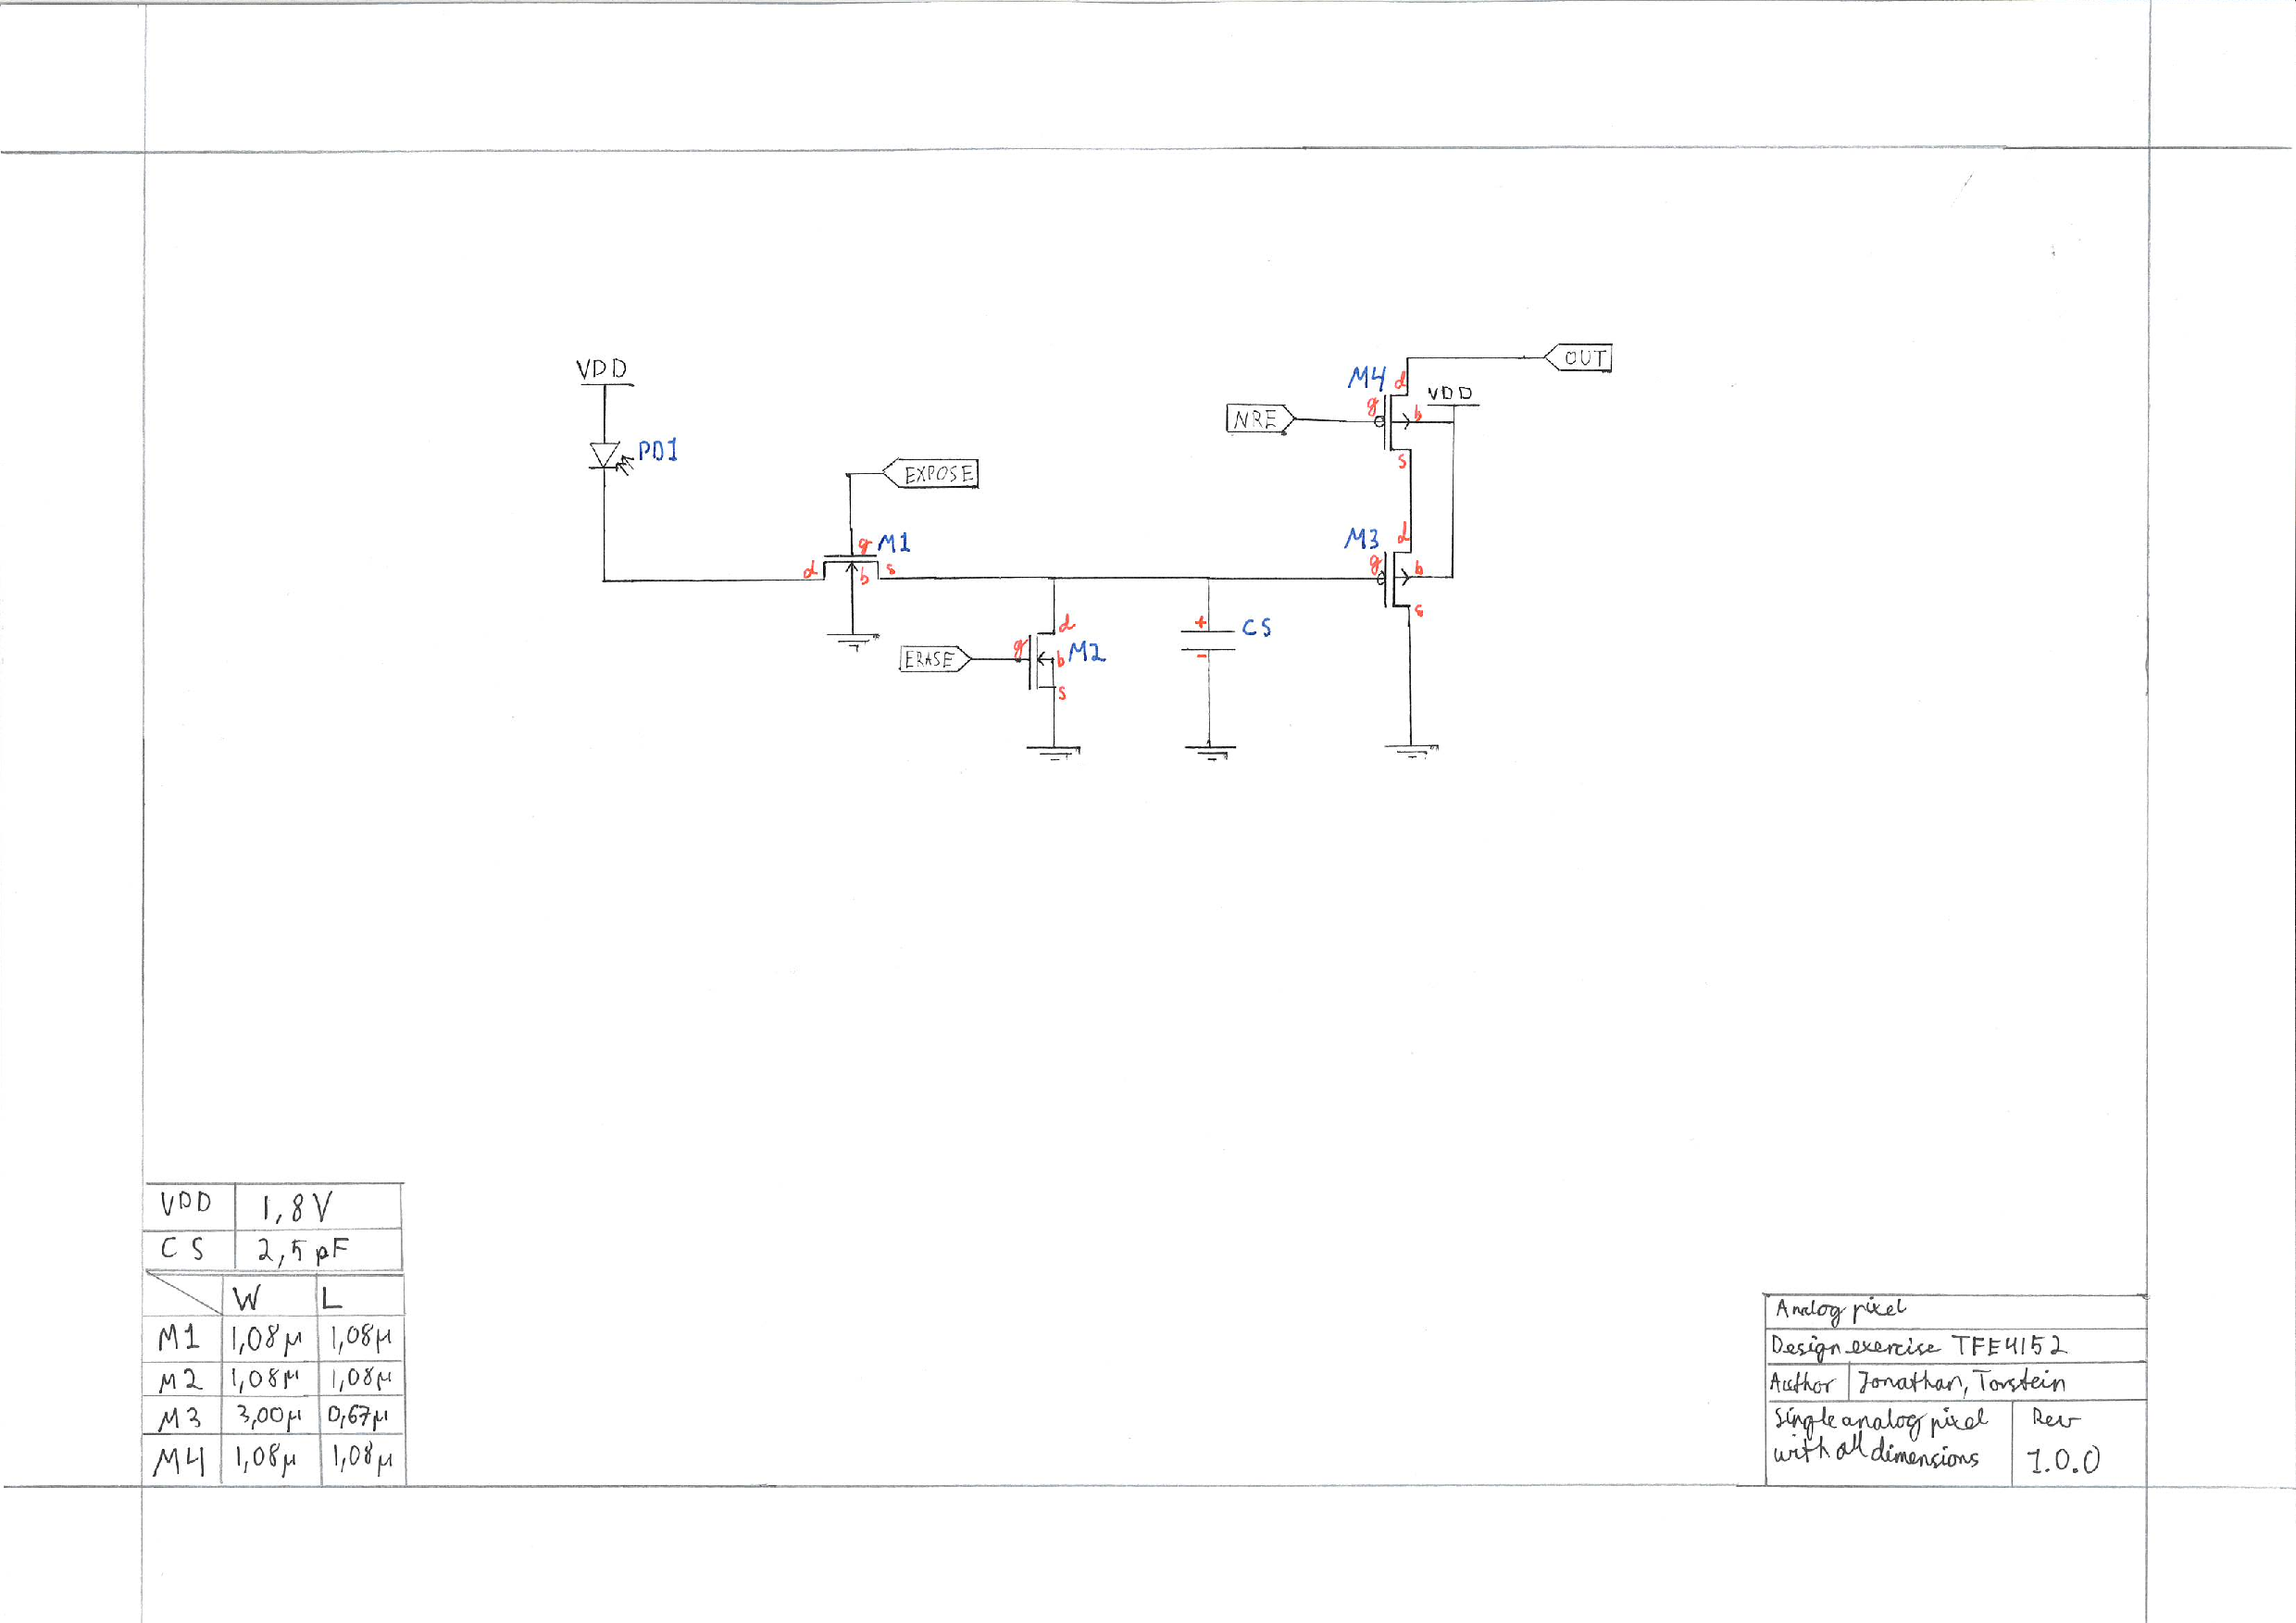
\includegraphics[width=0.85\textwidth]{figures/SchematicPixel}
  \caption{Schematic of one pixel with readout circuit, figure also exists bigger in Appendix~\ref{ap:Schematics}}\label{fig:pixelschematic}
\end{figure}


M3 is used to convert the voltage stored over CS into a variable resistance between N3 and VSS for a nondestructive readout of the pixel,
M4 functions as a simple switch to isolate the pixel from OUT to free the wire when other pixels in the camera are using it.



\subsection{Leakage through transistors}

We will in this project assume that all voltage transient are so slow that no leakage current is present between gate and the other ports of any of the transistors,
in the same way we assume there are no leakage currents through any of the capacitors.

As described in Analog~integrated~circuit~design~\cite{AnalogBook} the current from drain to source $I_D \propto \frac{W}{L}$.
This also makes sense from a geometric point of view.

In order to minimize the leakage current through a transistor that is shut off $\frac{W}{L}$ should be minimized.

\subsection{Conceptual workings of a camera controller}

As shown in Appendix~\ref{ap:Schematics}~figure~\ref{fig:analogCamera} the pixels depend on several digital input signals,
the job of the camera controller is therefore to trigger these in the desired order.
The requirements to be met by the controller are as follows:

\begin{itemize}
\item Pull the erase pin high except when exposing or reading the image
\item Pull the expose pin high for an appropriate length of time as defined by the user
\item Read out the values of all pixels in the correct order avoiding interference between different pixels on the same ADC.
\item Enable the user to reset the whole system. Though the image being taken might be lost the camera should function normally afterwards.
\end{itemize}


\newpage
\section{Analog design} \label{sec:AnalogDesign}
When designing the analog circuitry the topology as well as the technological limitations for production was taken from~\cite{oppgave}.
This section therefore focuses on the physical dimensions of the different components as specified in figures~\ref{fig:implpixel}~and~\ref{fig:implcamera}.

The most important property of the analog pixel is that the charge stored over CS remains unchanged while being read,
the transistors M1 and M2 must therefore be tuned for minimal leakage current as described in Section~\ref{sec:leakagecurrent}.
The transistor M4 must be tuned in the same way to avoid any interference between P11 and P21 as well as between P12 and P22 during readout as shown in figure~\ref{fig:implcamera}.

The current source transistors MC1 and MC2 must be tuned for the quickest possible response of the current source, this is in order to get the fastest possible stable output when reading from a pixel.
They are therefore tuned for maximum current throughput as explained in Section~\ref{sec:leakagecurrent} and verified in Section~\ref{sec:Simulations}.

The capacitor CS and transistor M3 are tuned to empirically found values as shown in Section~\ref{sec:Simulations} in order to give the best dynamic range of the pixel
as a function of lighting conditions and exposure time.

All component values are shown in table~\ref{tab:componentvalues}.

\begin{table}[htbp]
  \centering
  \caption{Physical values of components}
  \subcaption*{Panel A: transistors}
  \begin{tabular}{ c | c c }
    Component & W & L \\
    \midrule
    M1 & $1.08\mu$ & $1.08\mu$ \\
    M2 & $1.08\mu$ & $1.08\mu$ \\
    M3 & $3.00\mu$ & $0.67\mu$ \\
    M4 & $1.08\mu$ & $1.08\mu$ \\
    MC1 & $5.04\mu$ & $0.36\mu$ \\
    MC2 & $5.04\mu$ & $0.36\mu$
  \end{tabular}
  \bigskip
  \subcaption*{Panel B: capacitors}
  \begin{tabular}{c | c}
    Component & C \\
    \midrule
    CS & $2.5pF$ \\
    CC1 & $3.0pF$ \\
    CC2 & $3.0pF$
  \end{tabular} \label{tab:componentvalues}
\end{table}


\begin{figure}[htbp]
  \centering
  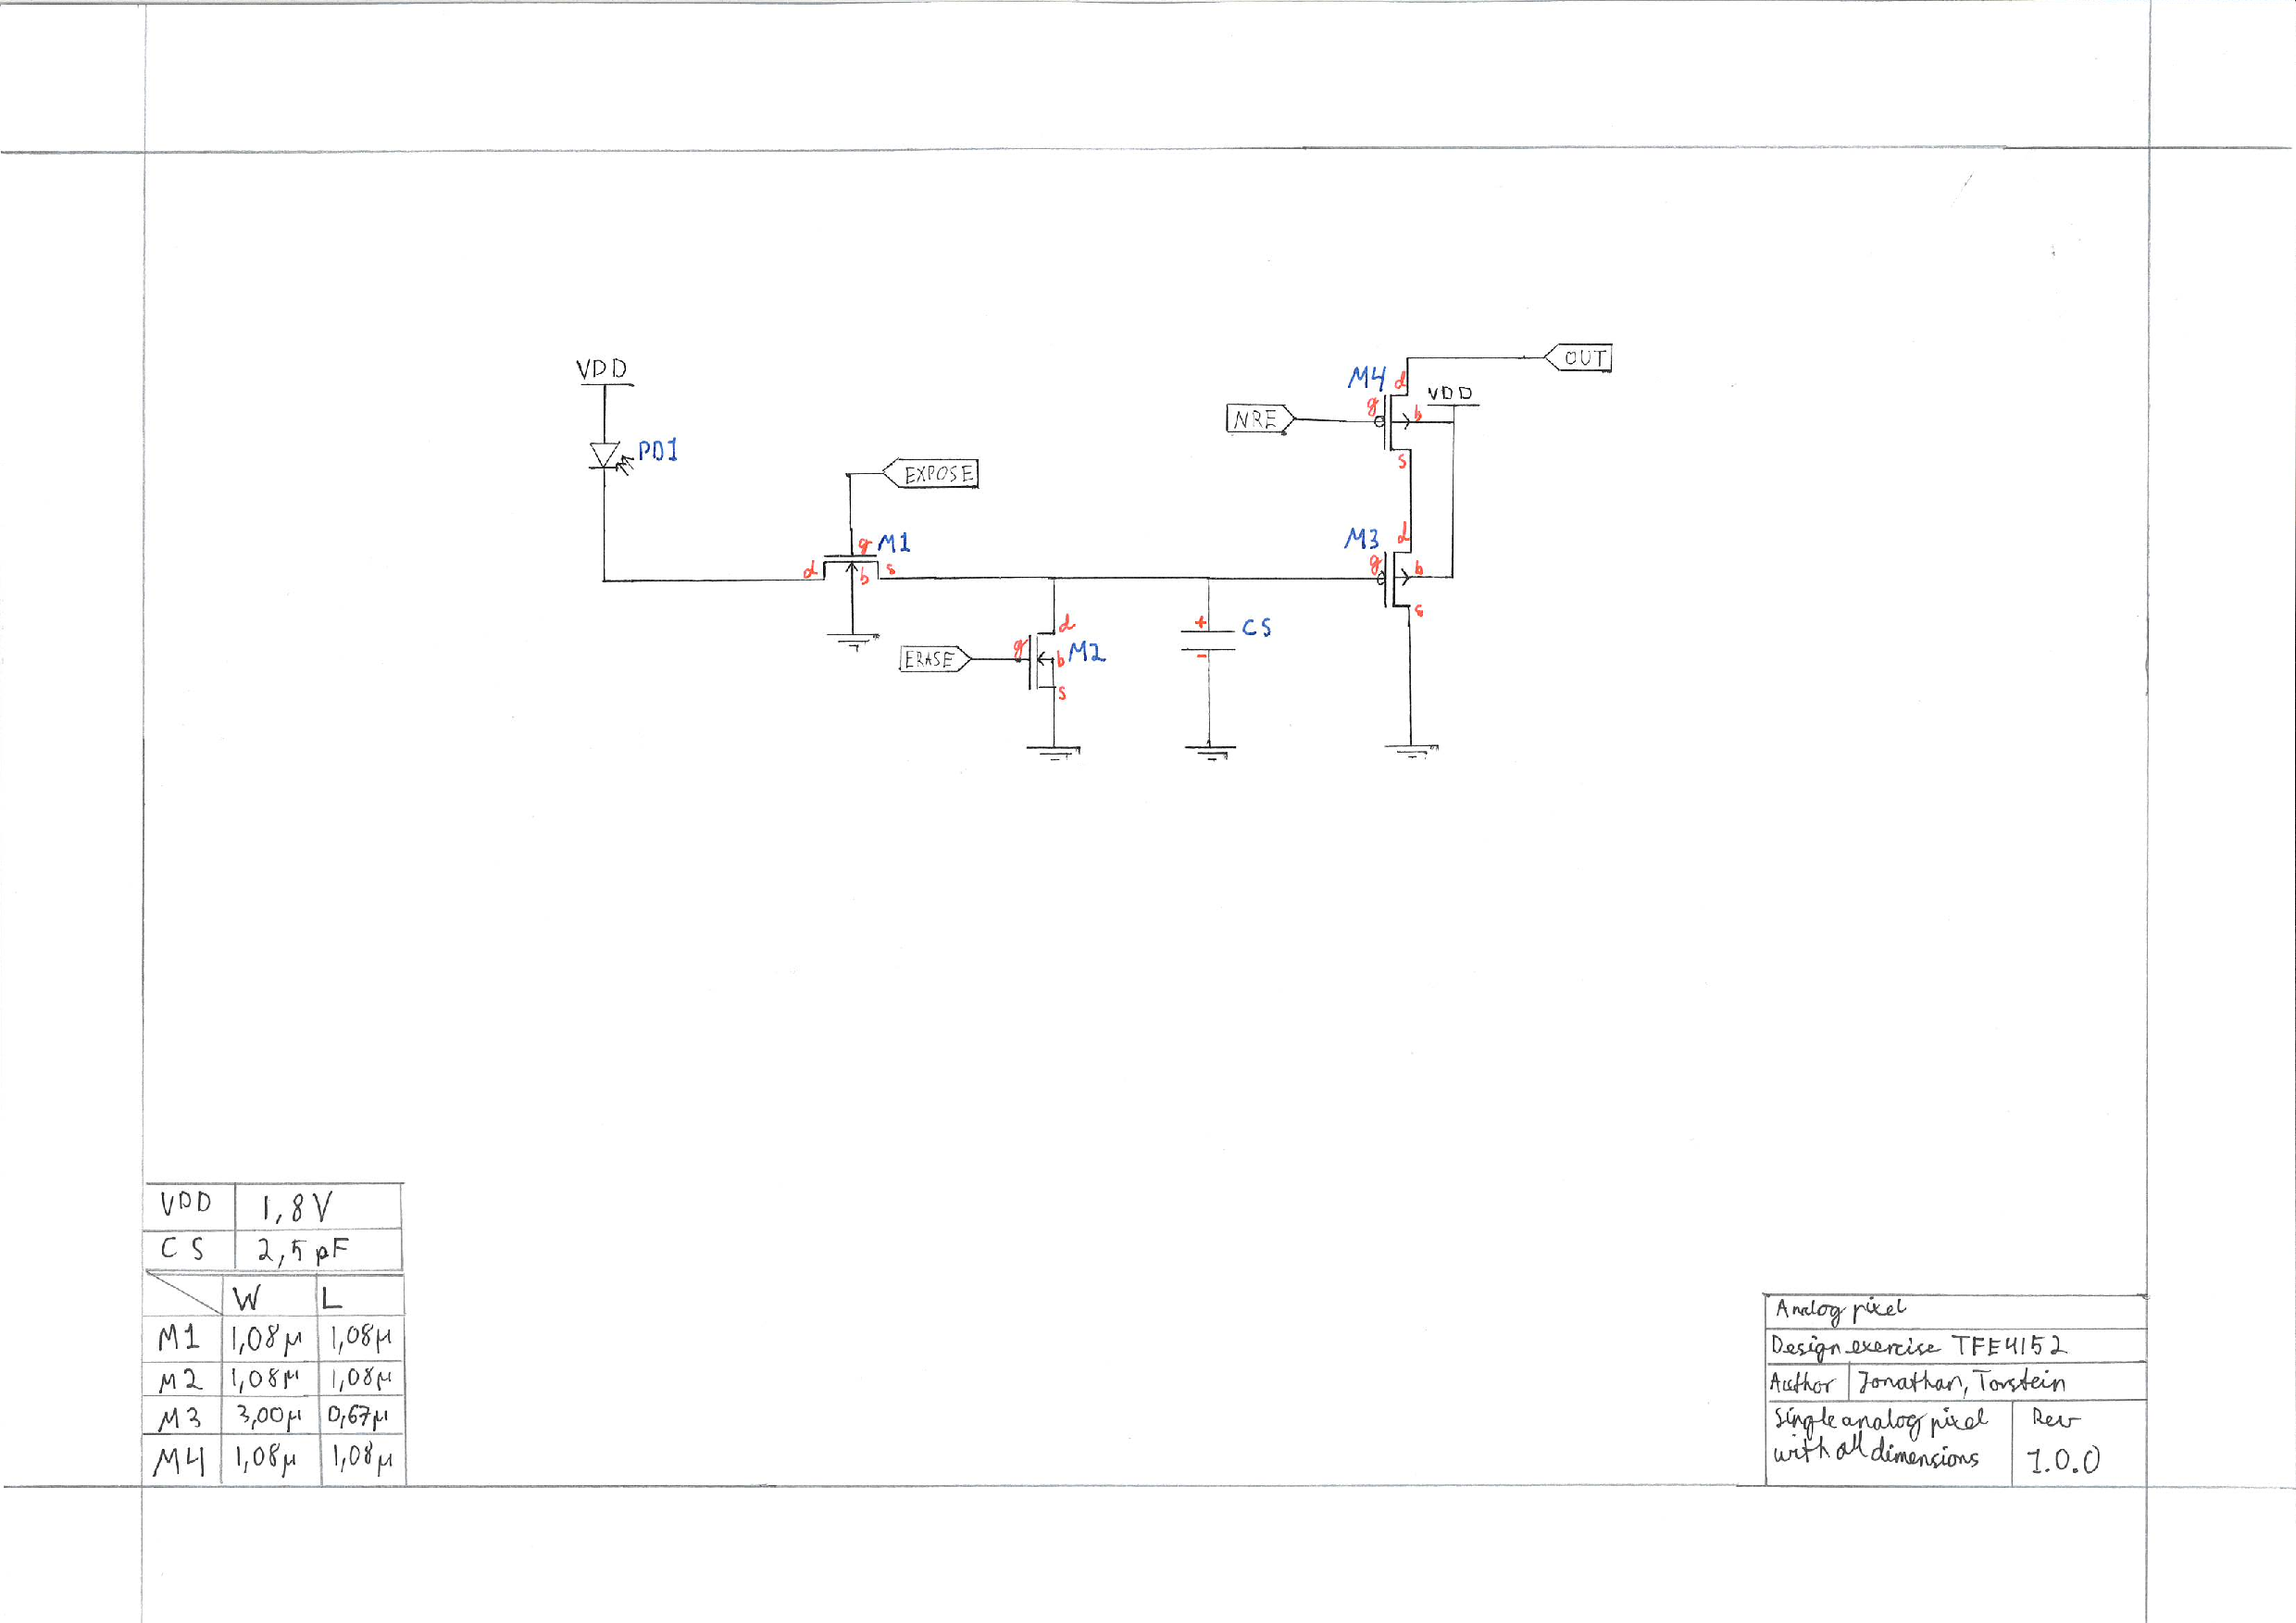
\includegraphics[width=0.85\textwidth]{figures/SchematicPixel}
  \caption{Implementation of one pixel, figure allso exist in Appendix~\ref{ap:Schematics}}
  \label{fig:implpixel}
\end{figure}
\begin{figure}[htbp]
  \centering
  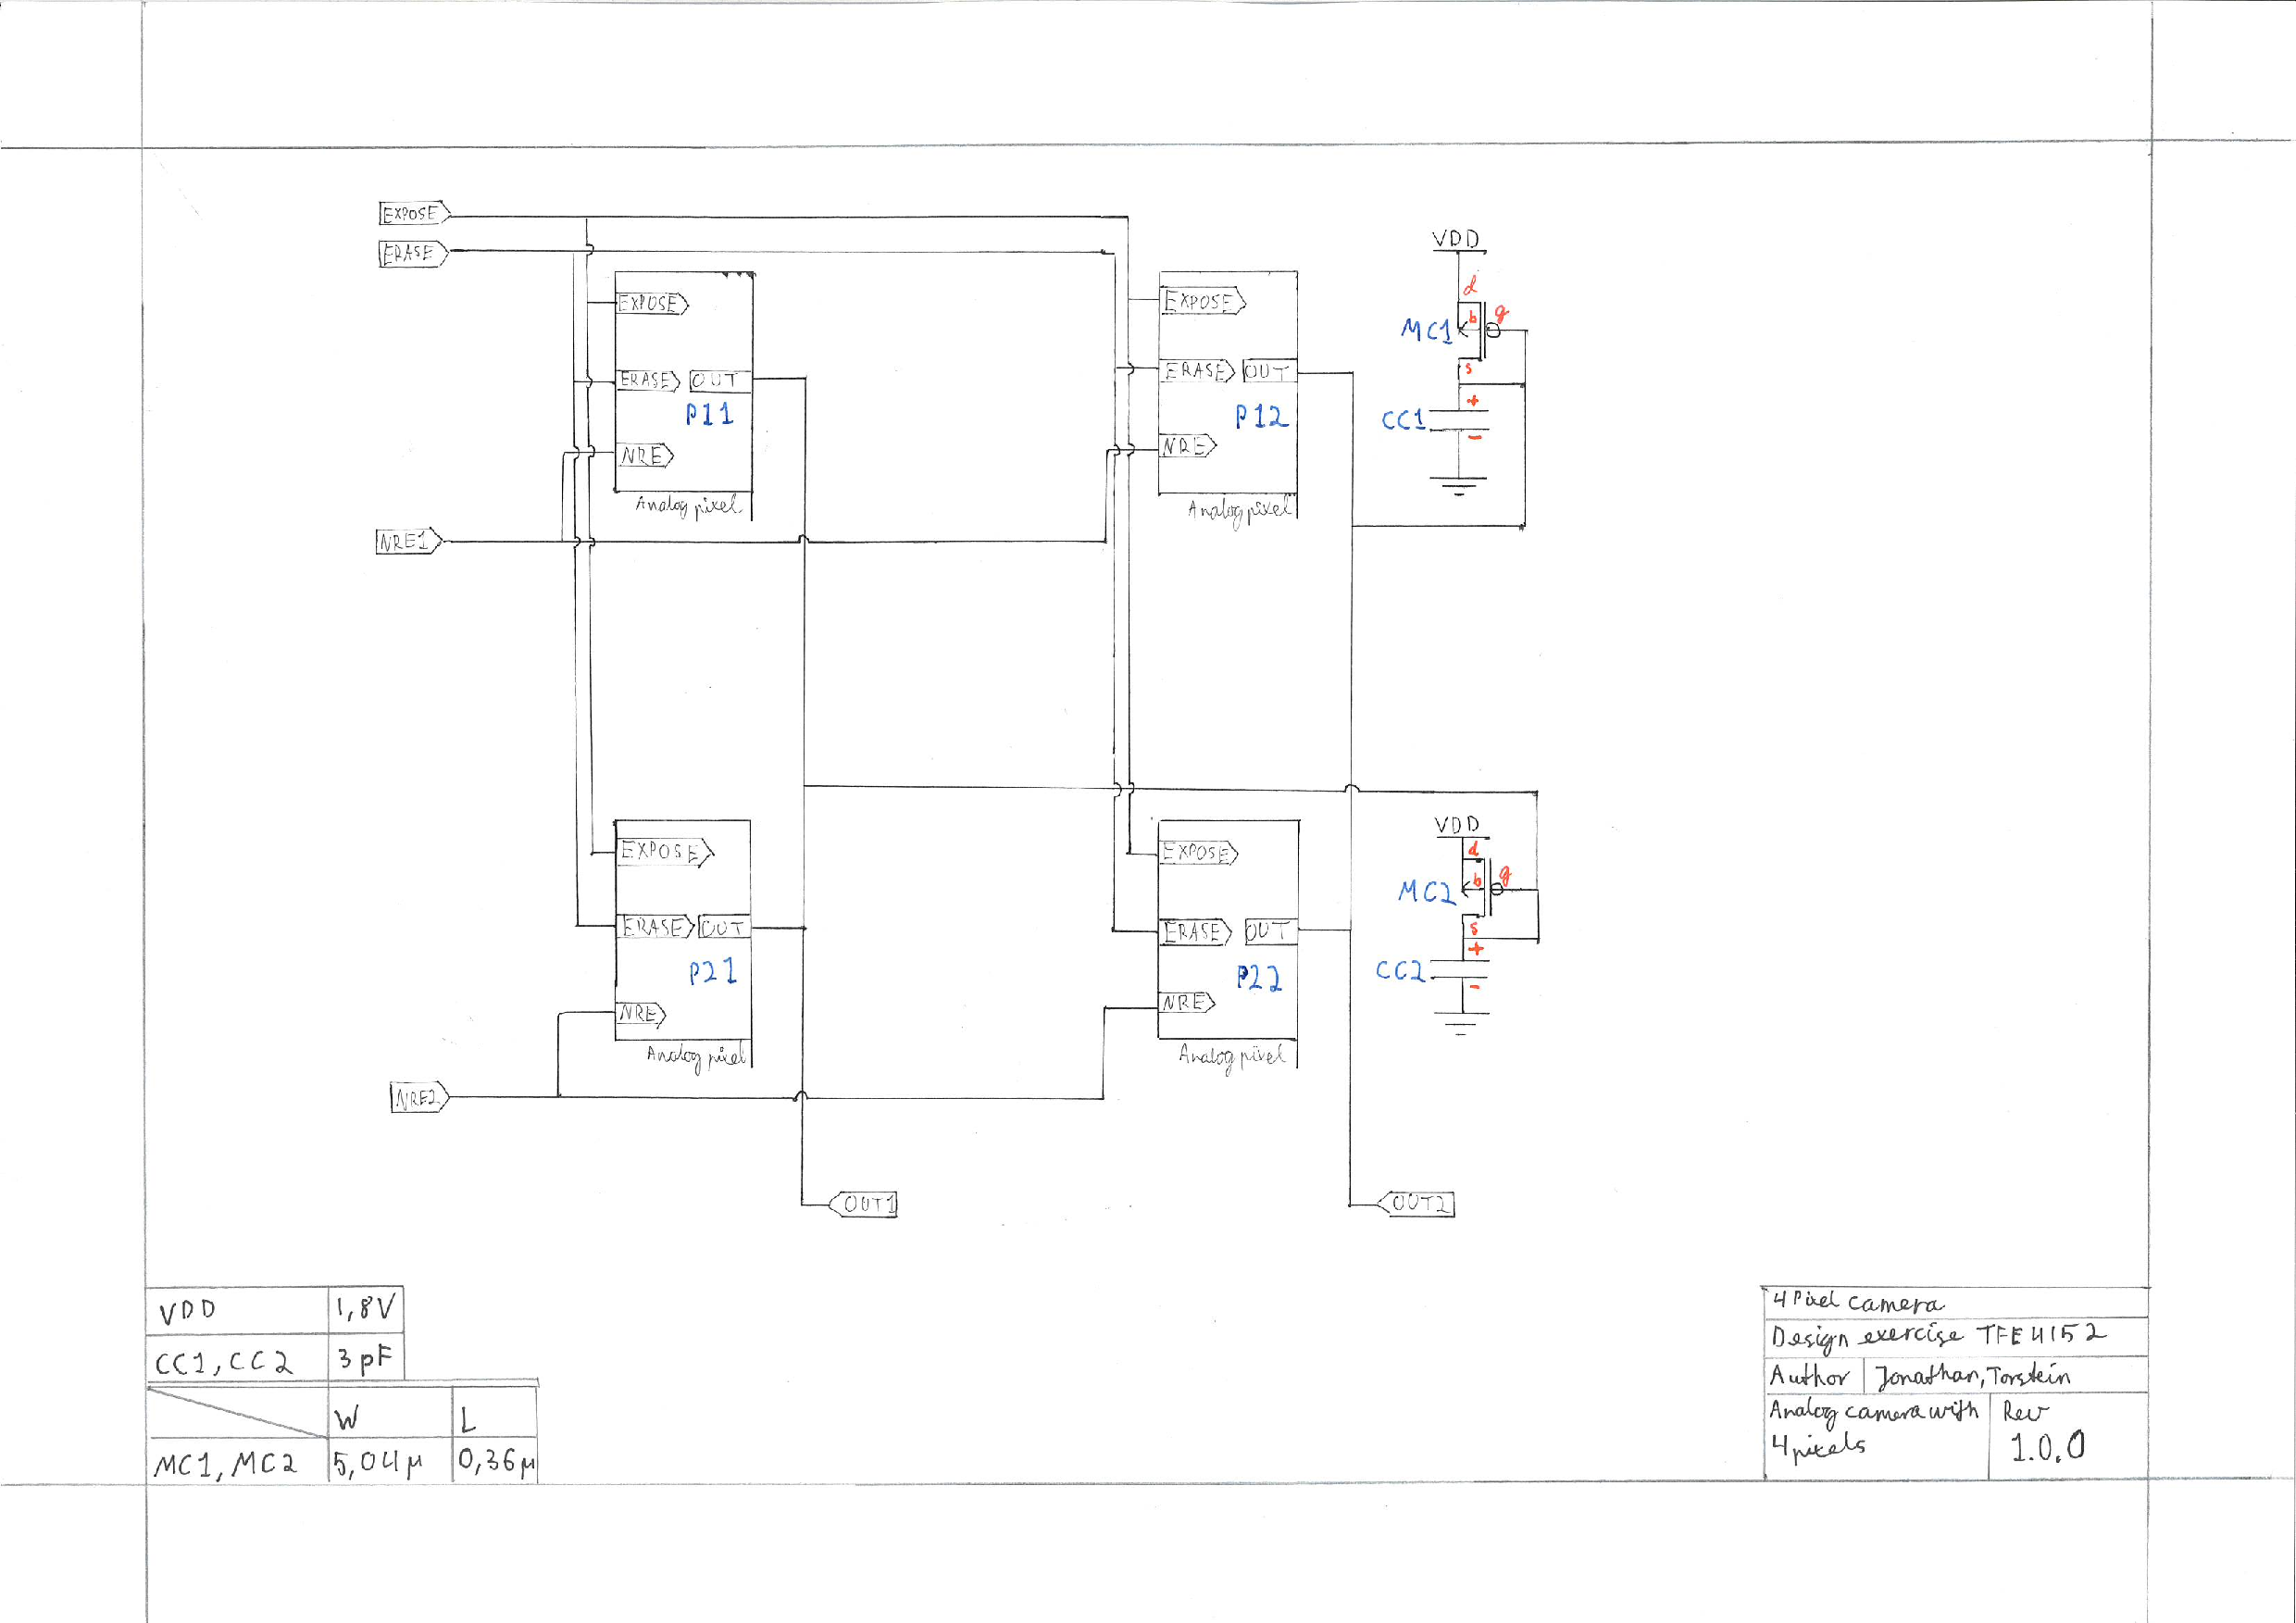
\includegraphics[width=0.85\textwidth]{figures/SchematicCamera}
  \caption{Implementation of the analog part of the camera, figure allso exist in Appendix~\ref{ap:Schematics}}
  \label{fig:implcamera}
\end{figure}

\newpage
\section{Digital design} \label{sec:DigitalDesign}
The design exists in appendix~\ref{ap:VerilogCode}.

\newpage
\section{Simulations} \label{sec:Simulations}
\subsection{Analog simulations}

All simulations of the analog circuitry were done using the AimSpice SPICE backend~\cite{AIMSpice} along with the AIMPlot~\cite{aimplot} frontend.


\subsection{Digital simulations}

All simulation of the digital control system were run using SystemVerilog testbenches in icarus~verilog~\cite{icarusVL} and shown in GTKWave~\cite{gtkwave}.

\newpage
\section{Conclusion} \label{sec:Conclusion}
This project has shown that dividing the camera into separate analog and digital parts is a good and efficient way of developing a design.
It has also been shown that a simple 4-pixel black and white camera can be implemented following this method.

The project has also developed many of the necessary buildingblocks for designing more complex digital cameras.

\newpage
\section{References} \label{sec:References}
\printbibliography



% ----------------------------------
% APENDIX
\newpage
\begin{appendices}
  
  % \section{First appendix}\label{ap:FirstAppendix}

  \section{Schematics} \label{ap:Schematics}
  \begin{figure}[H]
    \centering
    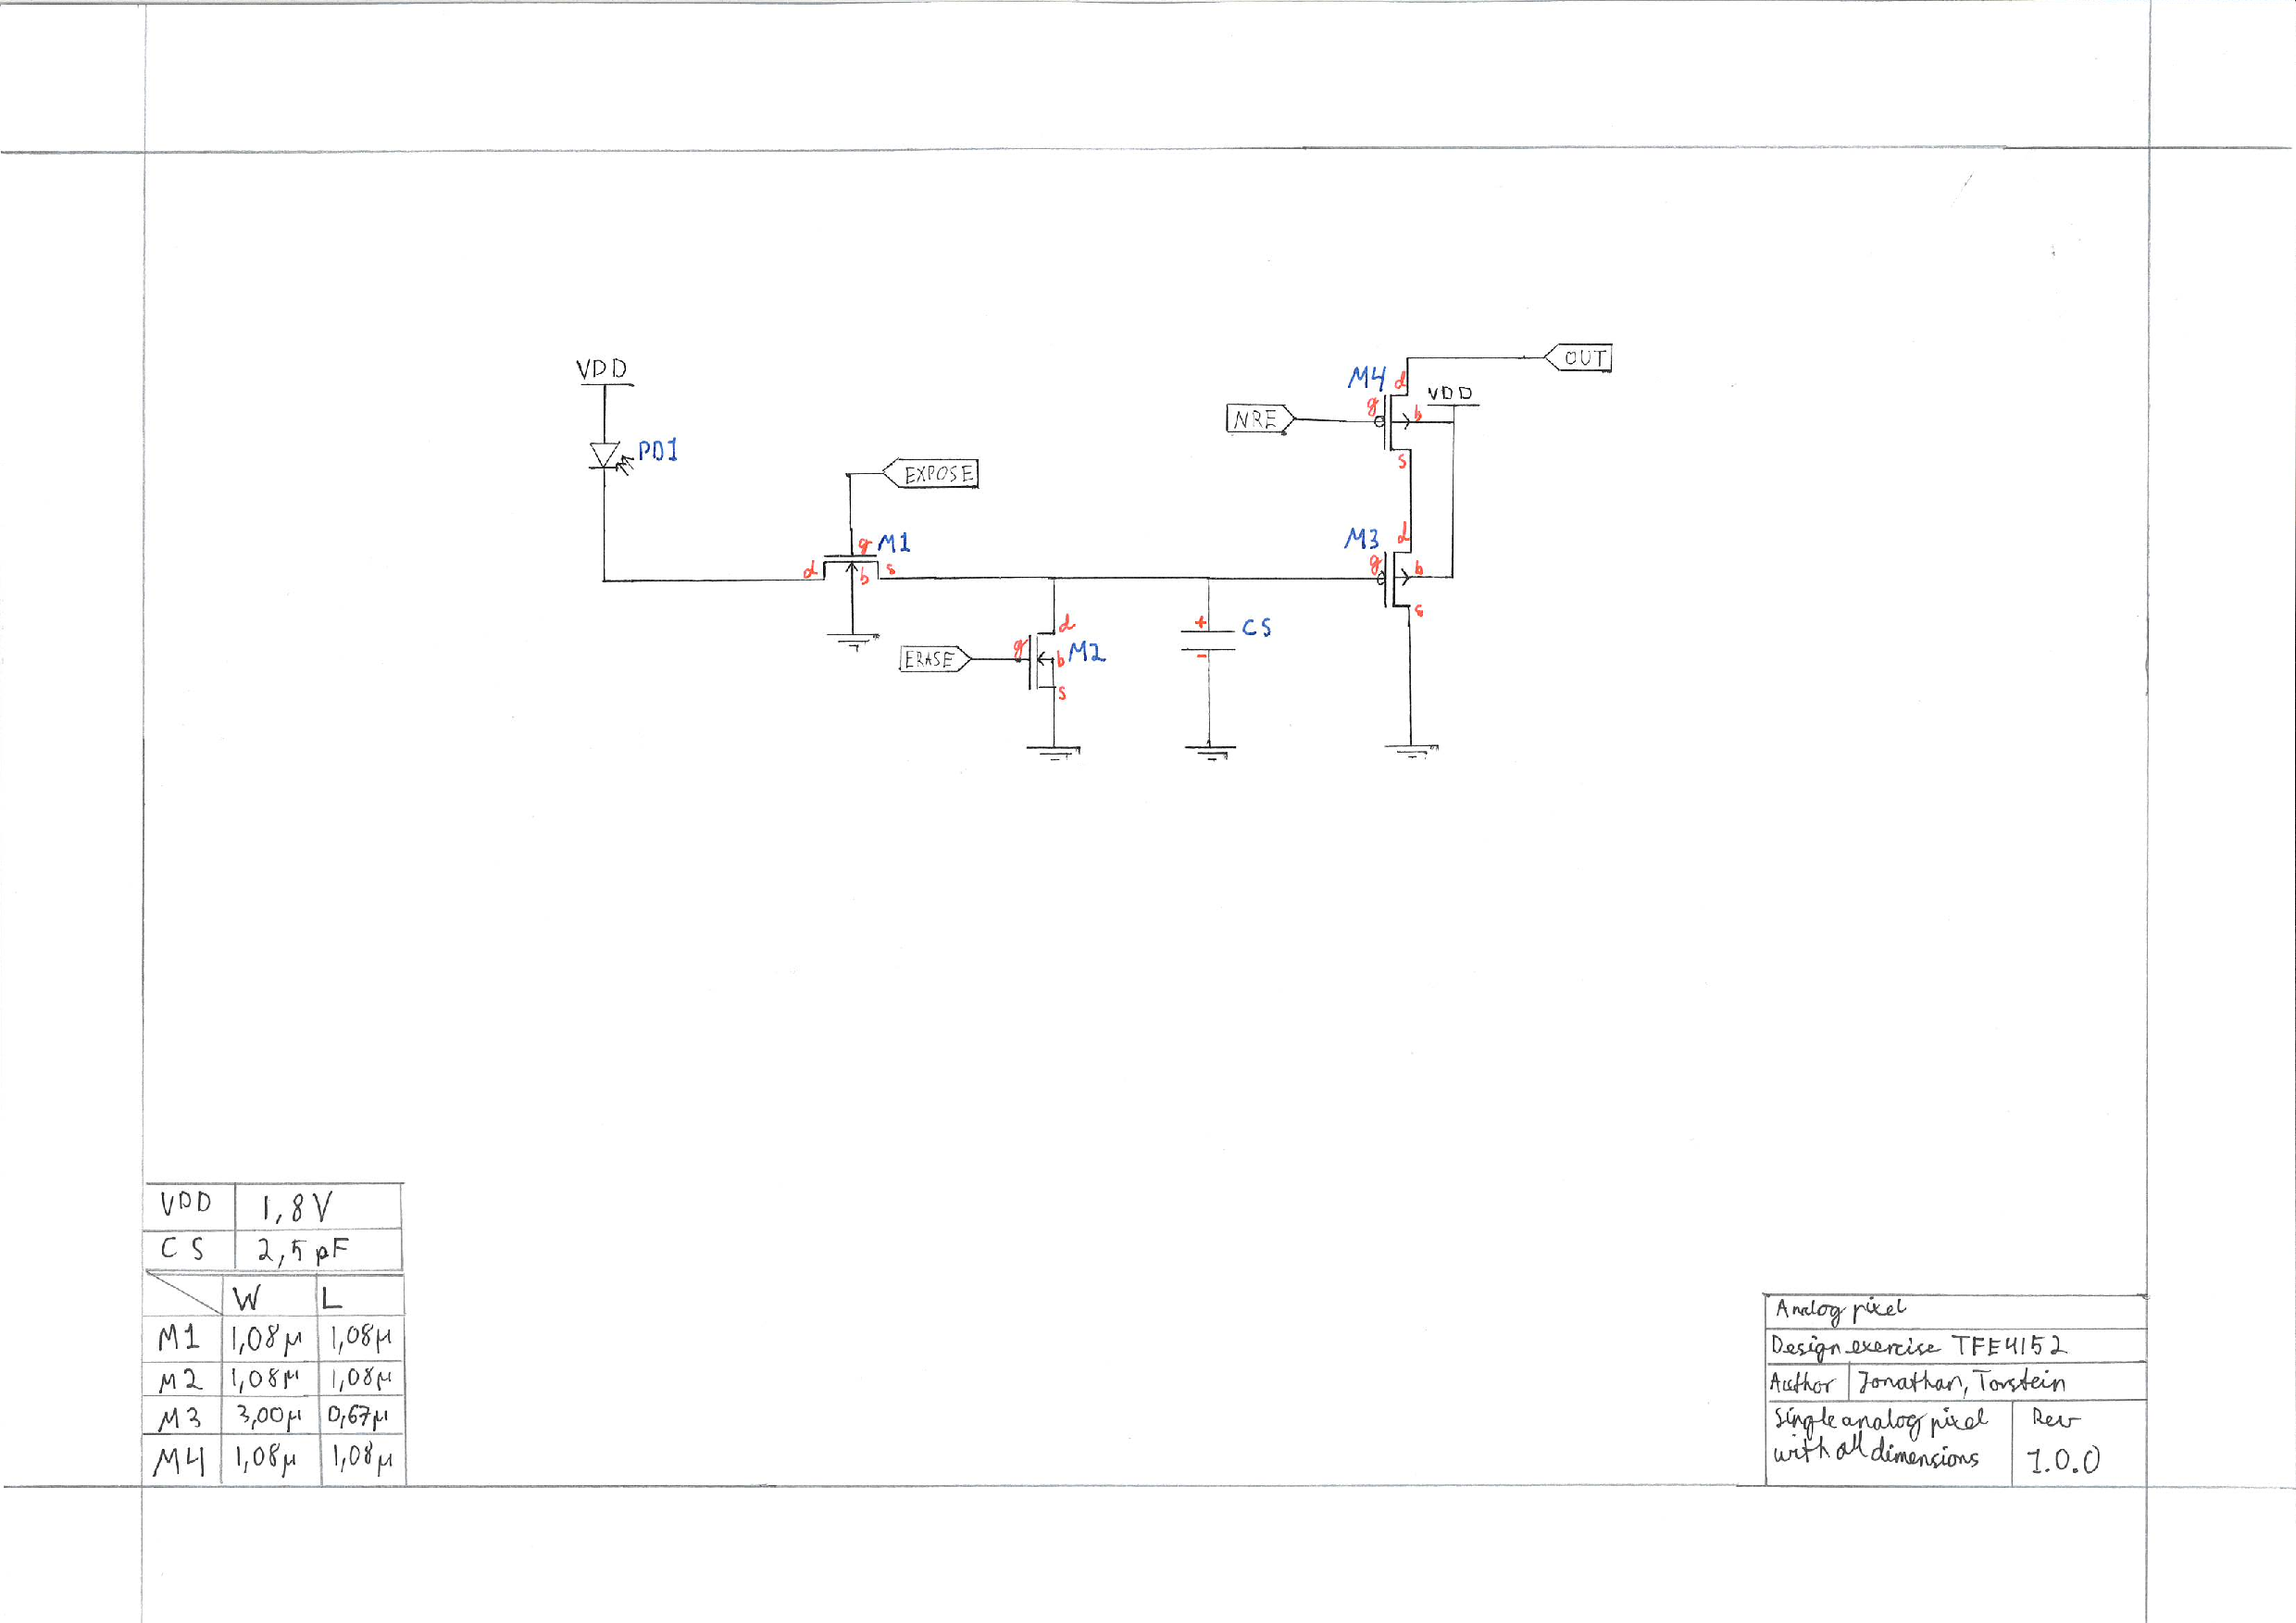
\includegraphics[angle=-90, scale=0.45]{figures/SchematicPixel.pdf}
    \caption{Analog schematic of one pixel}
    \label{fig:analogPixel}
  \end{figure}
  \begin{figure}[H]
    \centering
    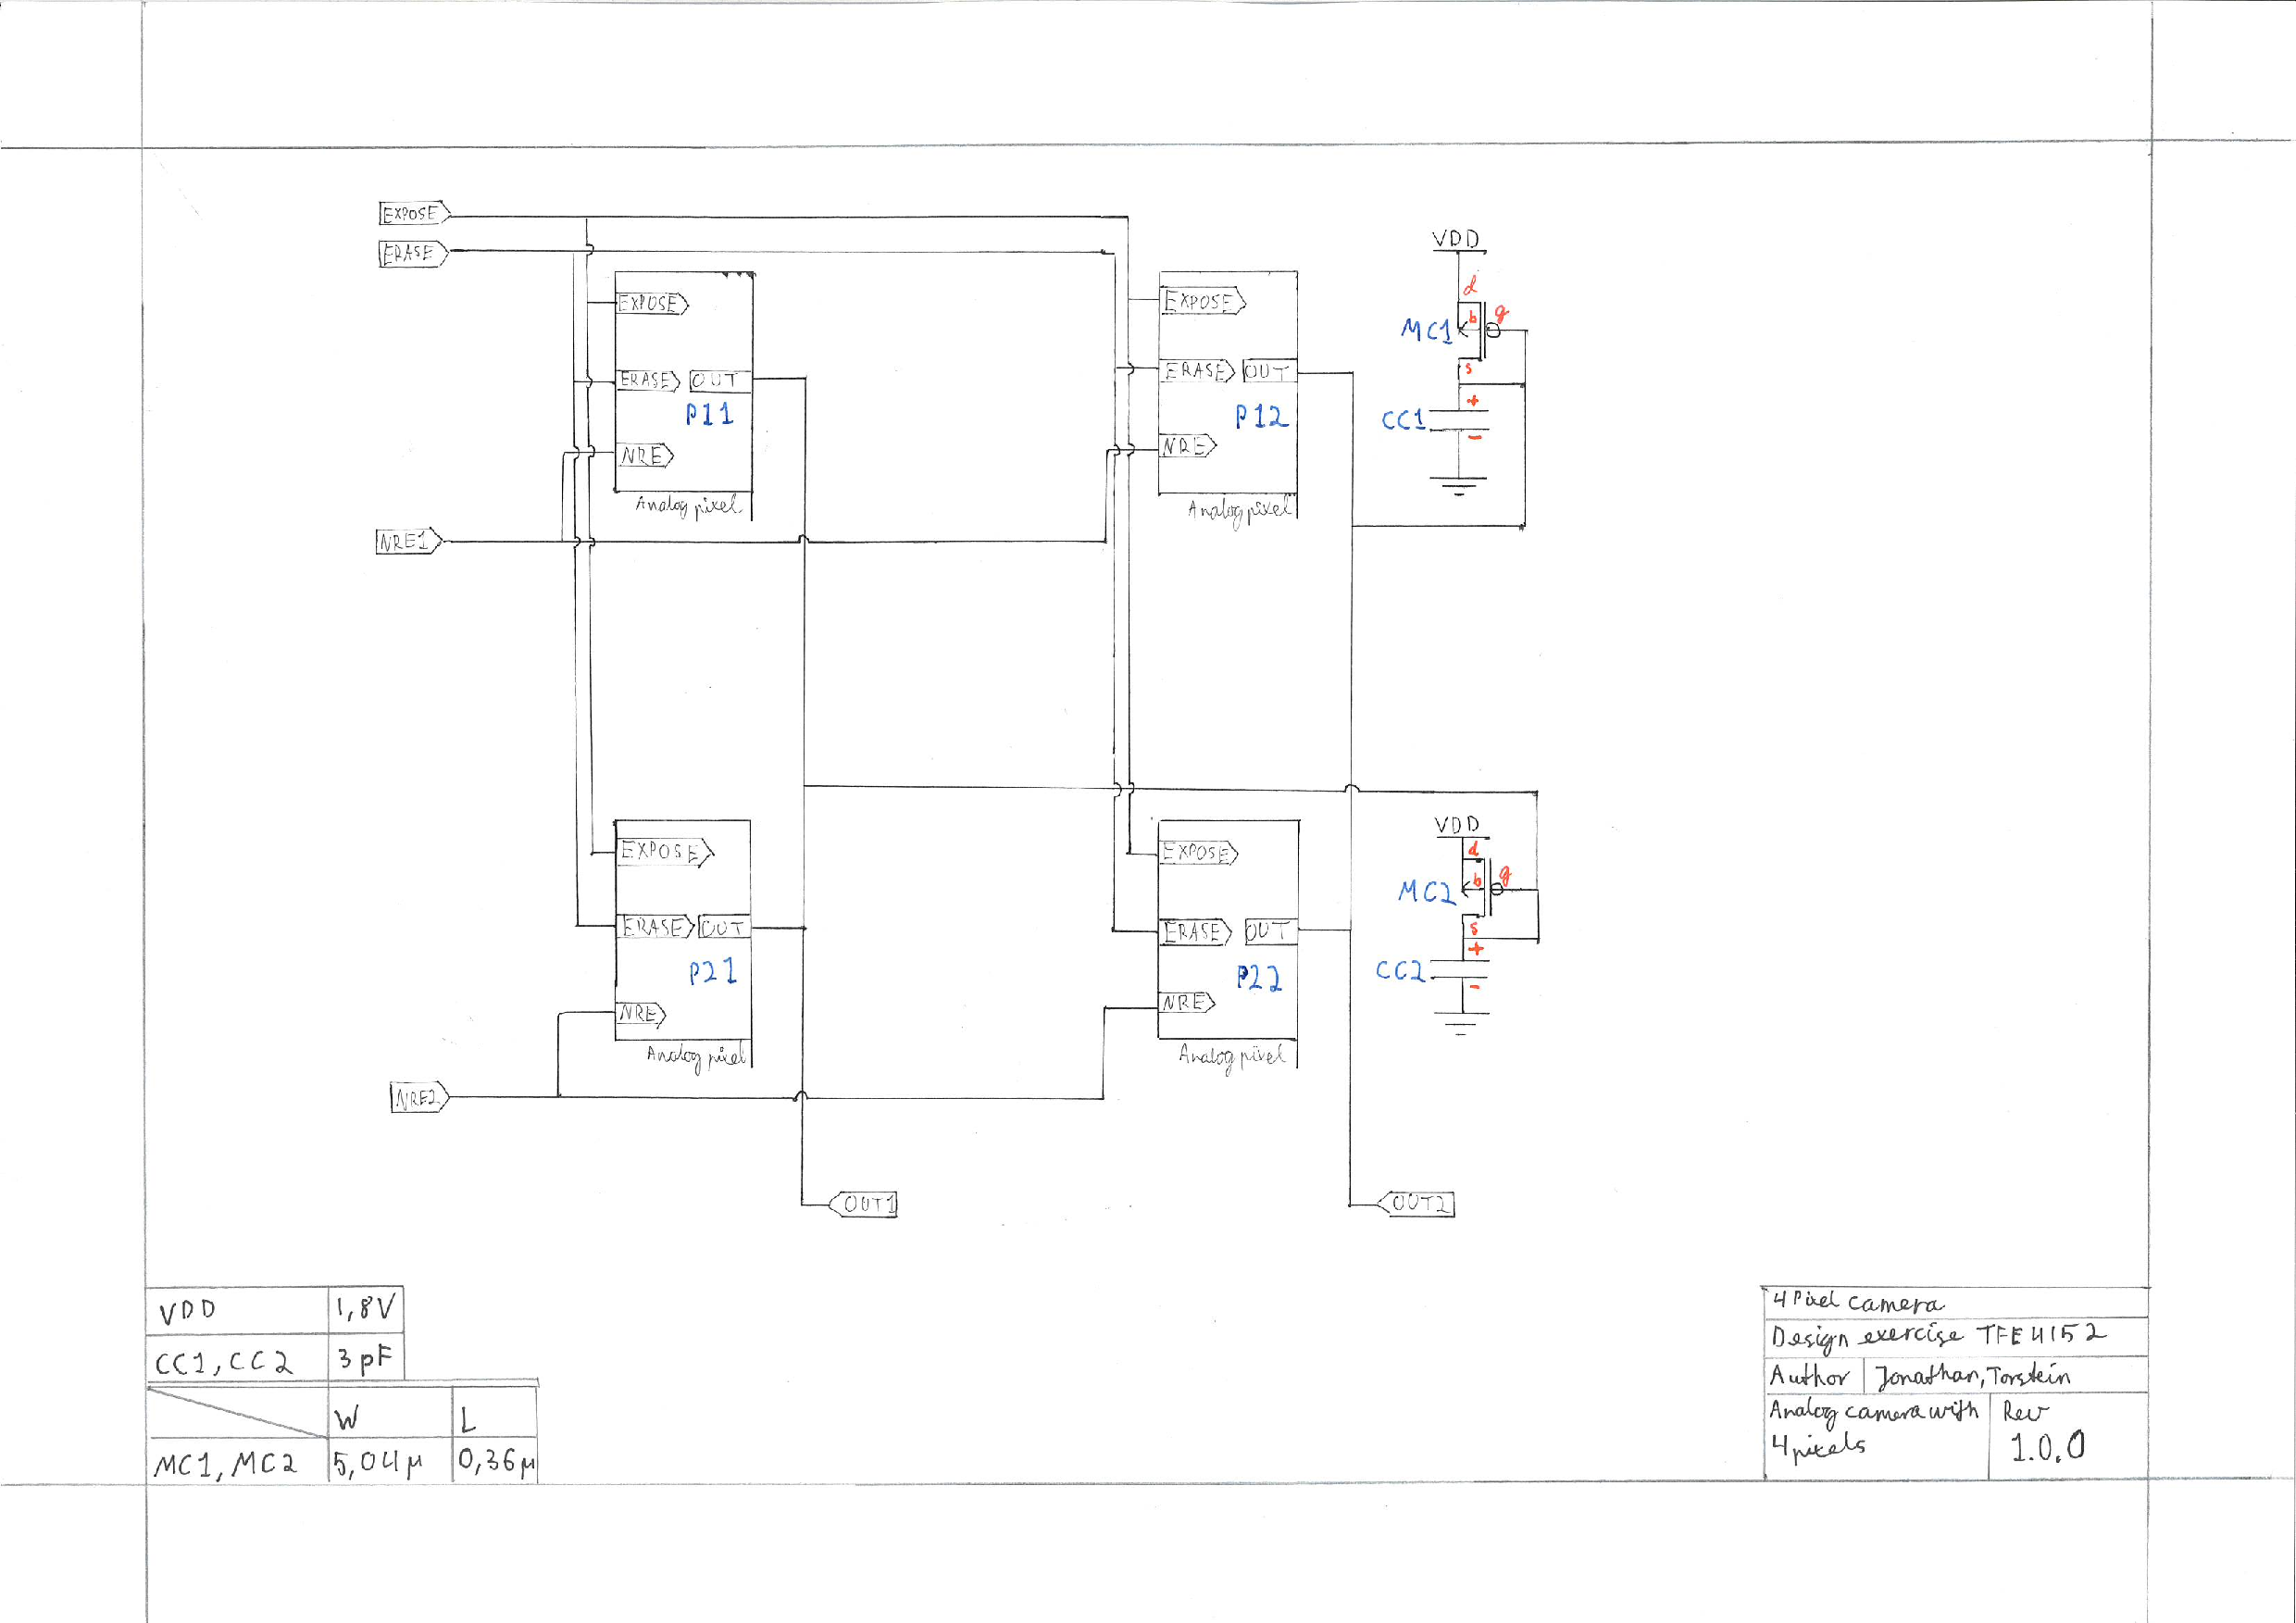
\includegraphics[angle=-90, scale=0.51]{figures/SchematicCamera.pdf}
    \caption{Analog schematic of 4 pixels in a camera}
    \label{fig:analogCamera}
  \end{figure}
  \begin{figure}[H]
    \centering
    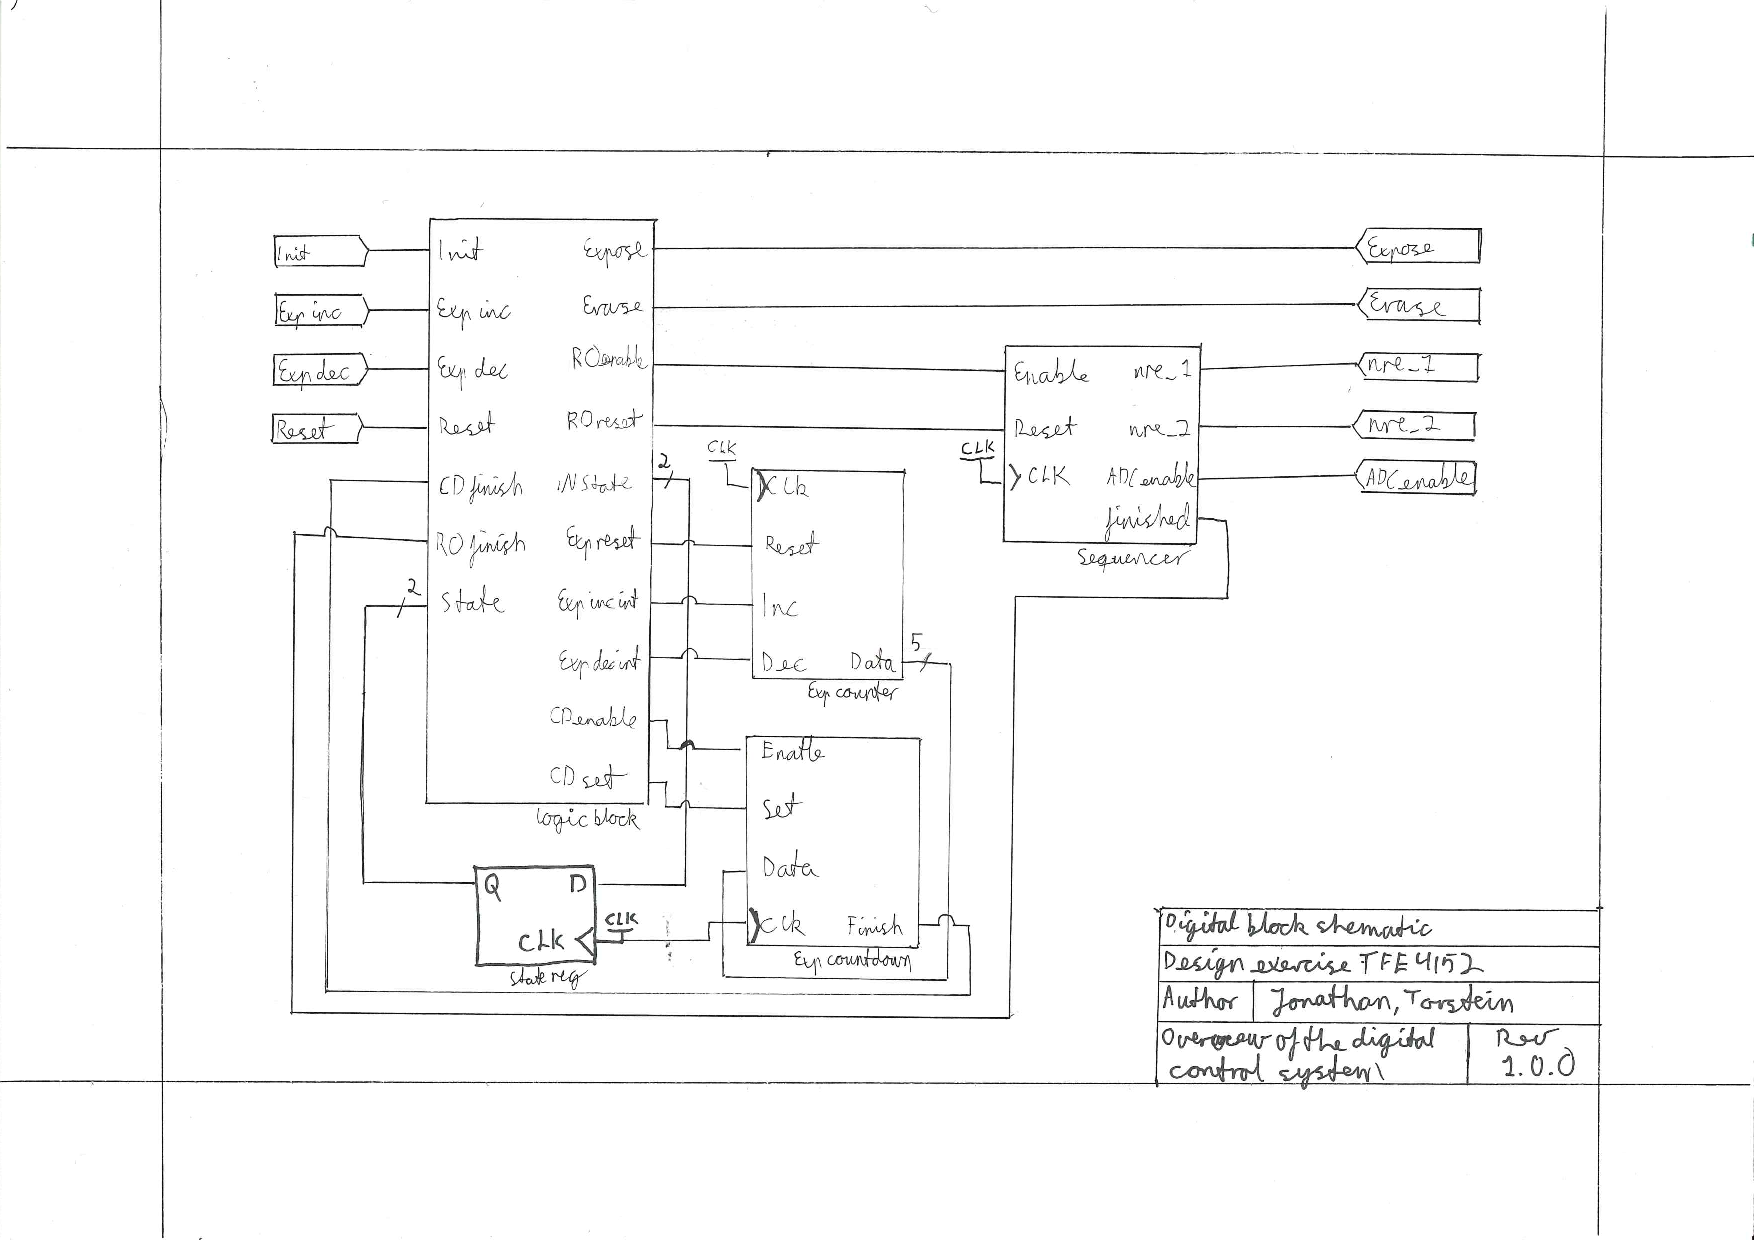
\includegraphics[angle=-90, scale=0.73]{figures/SchematicDigital}
    \caption{Digital schematic of the camera control}
    \label{fig:digitalControl}
  \end{figure}

  \newpage
  
  \section{Spice code} \label{ap:SpiceCode}
  \lstinputlisting[language=Verilog, caption={Main simulation of analog pixels}, label=ASCameraMain]{../analog/camera.cir}
  \lstinputlisting[language=Verilog, caption={Components in the camera}, label=ASComponents]{../analog/components.cir}
  \lstinputlisting[language=Verilog, caption={Parameters for the camera}, label=ASParameters]{../analog/parameters.cir}
  \lstinputlisting[language=Verilog, caption={MOSFET models part 1}, label=ASMosfet1]{../analog/models/p18_cmos_models.inc}
  \lstinputlisting[language=Verilog, caption={MOSFET models part 2}, label=ASMosfet2]{../analog/models/p18_model_card.inc}
  \lstinputlisting[language=Verilog, caption={Photo diode models}, label=ASPhotoResistor]{../analog/models/photo_diode.inc}
  
  \newpage
  
  \section{Verilog code} \label{ap:VerilogCode}
  \lstinputlisting[language=Verilog, style={verilog-style}, caption={Main module for camera control testbench}, label=VLCameraMainTB]{../digital/camera_fsm_tb.v}
  \lstinputlisting[language=Verilog, style={verilog-style}, caption={Main module for camera control}, label=VLCameraMain]{../digital/camera_fsm.v}
  \lstinputlisting[language=Verilog, style={verilog-style}, caption={Exposure register}, label=VLExpReg]{../digital/exp_reg.v}
  \lstinputlisting[language=Verilog, style={verilog-style}, caption={Counter for exposure time}, label=VLFCD]{../digital/fcd_reg.v}
  \lstinputlisting[language=Verilog, style={verilog-style}, caption={Readout sequencer}, label=VLSeq]{../digital/readout_seq.v}
  
\end{appendices}
\end{document}

